\setlength{\columnsep}{3pt}
\begin{flushleft}
	There are 3 permission available for all types of files:
	\begin{figure}[h!]
		\centering
		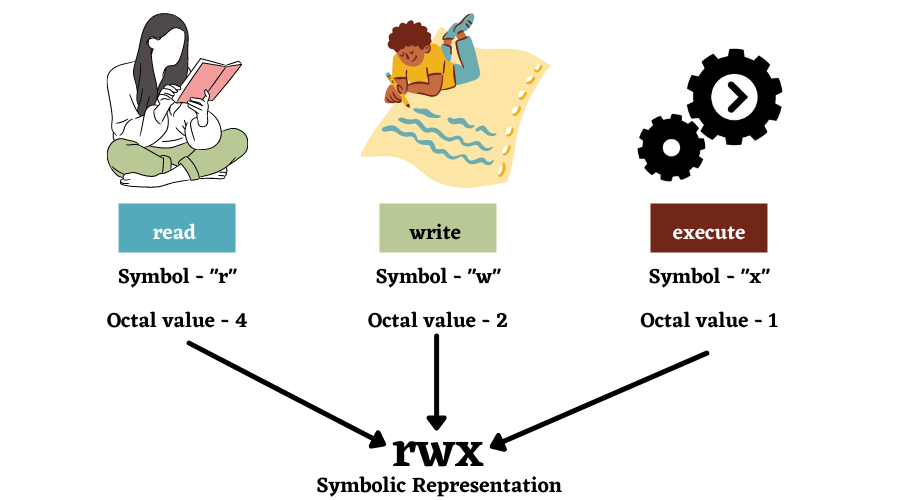
\includegraphics[scale=0.5]{content/chapter5/images/perm2.png}
		\bigskip
		\caption{File Permission}
		\label{fig:file_permission}
	\end{figure}

	Let's see what does this means for a normal file and directory.
	\newpage
	\paragraph{Read means:}
	\begin{figure}[h!]
		\centering
		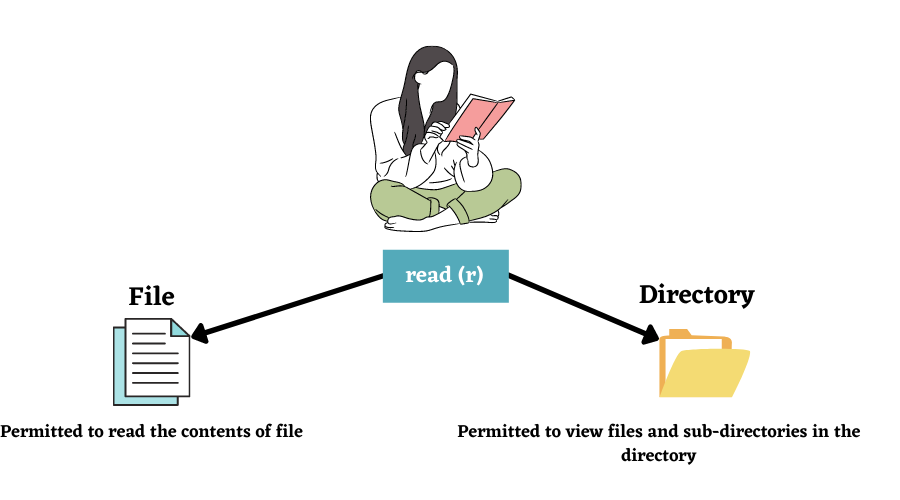
\includegraphics[scale=0.4]{content/chapter5/images/8.png}
		\caption{Read Permission}
		\label{fig:read_permission}
	\end{figure}

	\paragraph{Write means:}
	\begin{figure}[h!]
		\centering
		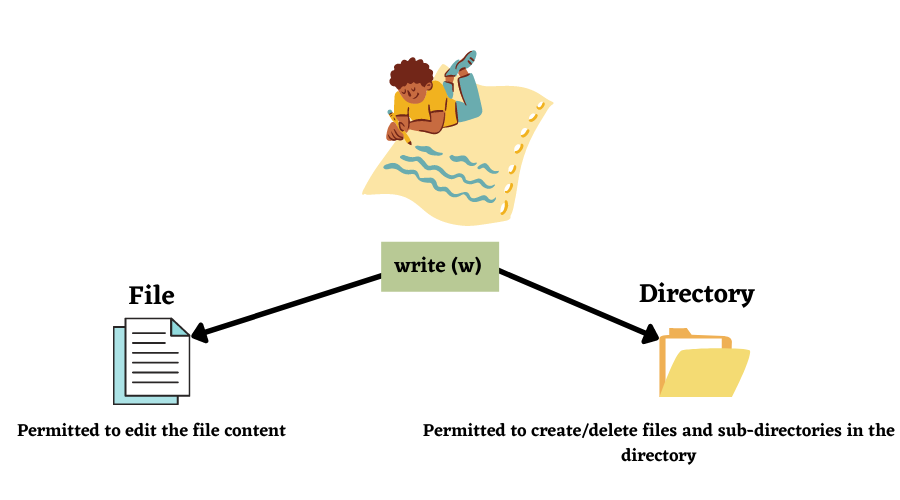
\includegraphics[scale=0.4]{content/chapter5/images/9.png}
		\caption{Write Permission}
		\label{fig:write_permission}
	\end{figure}

	\paragraph{Execute means:}
	\begin{figure}[h!]
		\centering
		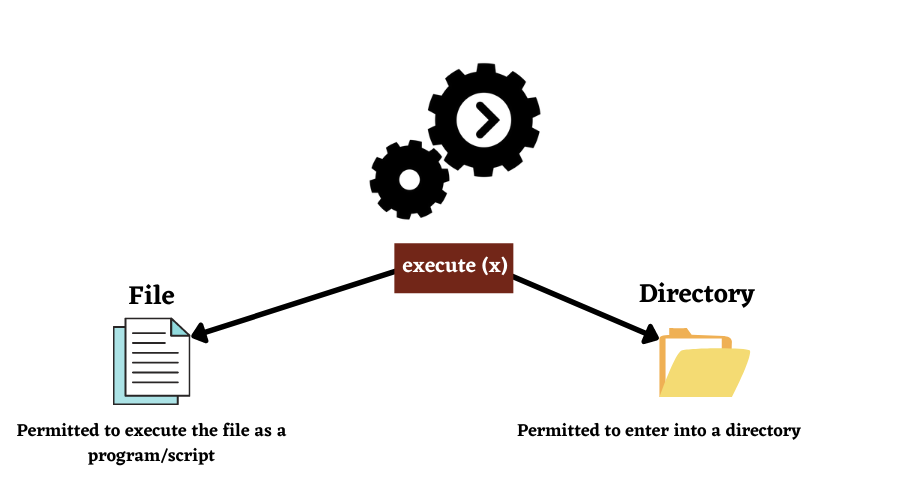
\includegraphics[scale=0.4]{content/chapter5/images/perm3.png}
		\caption{Execute Permission}
		\label{fig:execute_permission}
	\end{figure}



	
\end{flushleft}

\newpage

